\documentclass[a4paper,twoside,titlepage]{article}

%--- Packages ----------------------------------------------------------------
\usepackage{a4}
\usepackage[english]{babel}

\usepackage{rotating}

\usepackage[inner=2cm,top=2cm,outer=3cm,bottom=1cm,includehead,includefoot]{geometry}
\usepackage[latin1]{inputenc}
% \usepackage[utf8]{inputenc}
\usepackage{moreverb}
\usepackage{float}
\usepackage{graphicx}
%\usepackage{makeidx}
%\makeindex
% Don't forget to run makeindex and include \printindex
\usepackage{fancyhdr}
 \usepackage[colorlinks=true,linkcolor=black,urlcolor=black]{hyperref} % Reference by title

\setcounter{tocdepth}{2} % Only subsections in toc

%--- Definitions -------------------------------------------------------------

\def\author			{}
\def\course			{5EL011 VT10}
\def\coursename	    {Embedded Systems}
\def\delivery		{Project 2 Report}
\def\version		{1.0}
\def\trivialname	{Project 2}
\def\tutor			{}


% New output float
\floatstyle{boxed}
\newfloat{program}{thp}{lop}
\floatname{program}{Program}
\newfloat{output}{thp}{lop}
\floatname{output}{Output}

%\restylefloat{figure}

 \hypersetup{
 pdfauthor = {\author},
 pdftitle = {\trivialname{} - \delivery},
 pdfsubject = {\coursename},
 pdfkeywords = {umu, edu, c, avr}
 }


\newcommand{\HUGE}{\fontsize{36}{42}\selectfont{}}
\newcommand{\helvetica}{\fontfamily{phv}\selectfont}
\newcommand{\degree}{\ensuremath{^\circ}}
\pagestyle{fancy}
	\lhead[\coursename]{\today}
	\chead[\textsc{\trivialname~- \delivery}]{\textsc{\trivialname~- \delivery}}
	\rhead[\today]{\course}
	
	\lfoot[\thepage]{\author}
	\cfoot[]{}
	\rfoot[\author]{\thepage}
	
	\renewcommand{\headrulewidth}{0.4pt} 
	\renewcommand{\footrulewidth}{0.4pt}

%-----------------------------------------------------------------------------
\begin{document}
\pagestyle{empty}
%--- Titlepage ---------------------------------------------------------------
\begin{titlepage}
	{
	\helvetica
	\begin{flushright}
		\small \coursename{} \course\\
	\end{flushright}
	\begin{center}
		\LARGE \trivialname\\
		\HUGE { \textbf{\delivery}} \\
		\small \textbf{\author}\\
		\normalsize {
			Emil Eriksson (\href{mailto:c07een@cs.umu.se}{\texttt{c07een@cs.umu.se}}) \\
			Rickard Westerlund (\href{mailto:c07rwd@cs.umu.se}{\texttt{c07rwd@cs.umu.se}})
    		}
	\end{center}
	\vfill
	\begin{flushright}
		\subsection*{Examinator}
		Nils-Erik Eriksson (\href{mailto: nilserik.eriksson@tfe.umu.se}{nilserik.eriksson@tfe.umu.se})
	\end{flushright}
	}
\end{titlepage}

\pagestyle{fancy}
\pagenumbering{roman}
%--- Table of contents -------------------------------------------------------
\tableofcontents
\clearpage
\newpage

%--- Document ----------------------------------------------------------------
\pagenumbering{arabic}

\section{Introduction}

\section{Materials and Methods}

\section{Results}

\section{Discussion}

%referenslista
%  \bibliographystyle{plain}
%  \bibliography{plan}

    %%%%%%%%%%%%%%%% bilagor %%%%%%%%%%%%%%%%
    \clearpage
    \appendix
	\section{Wiring Diagram}\label{wiring-diagram}
	\begin{figure}[!htp]
        \centering
        %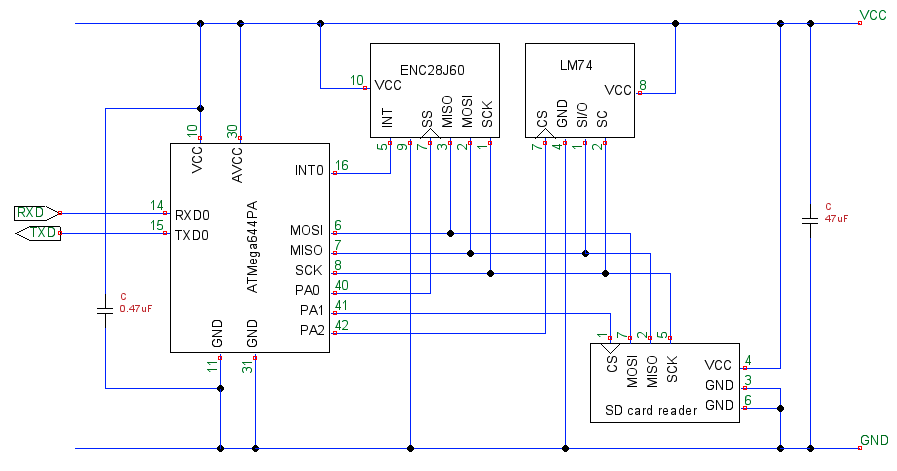
\includegraphics[width=\textwidth]{kopplingsschema.png}
        \caption{Wiring diagram}
        \label{fig:wiring-diagram}
    \end{figure}

	\section{Activity Diagram}\label{activity-diagram}
	\begin{figure}[!htp]
        \centering
        %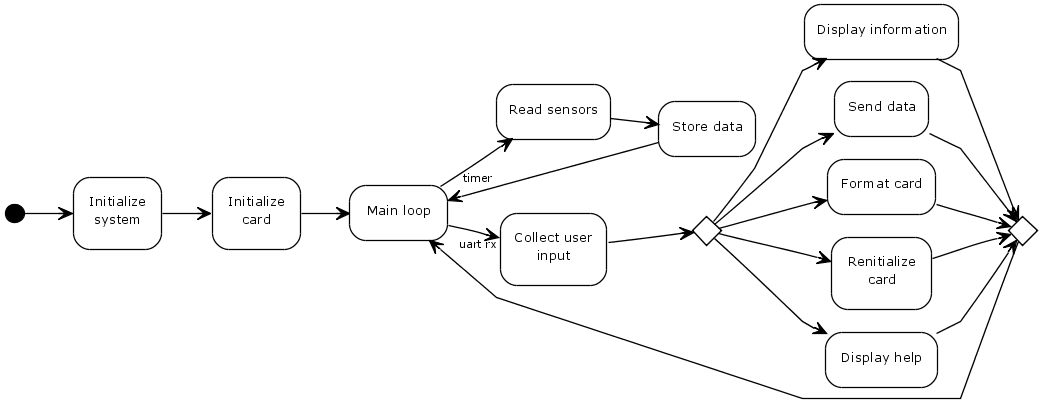
\includegraphics[width=\textwidth]{aktivitetsdiagram.png}
        \caption{Activity diagram showing how the program operates.}
        \label{fig:activity-diagram}
    \end{figure}

\end{document}
